%------------------------------------------------
\section{Chiffrement Asymétrique}
%------------------------------------------------

\begin{frame}
    \frametitle{Introduction}
    \begin{itemize}
        \item Méthode de chiffrement a deux clefs
        \item Ce qui est chiffré avec une clef ne peut être déchiffré que par l'autre
    \end{itemize}
    \begin{center}
        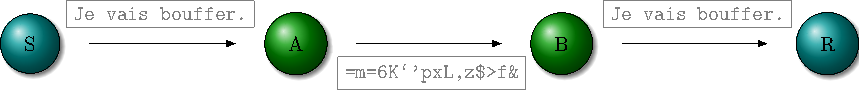
\includegraphics[scale=0.7]{res-src/asym_crypto}
        \vspace{4em}
        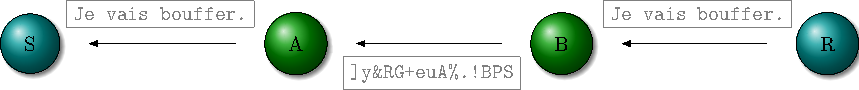
\includegraphics[scale=0.7]{res-src/asym_cryptor}
    \end{center}
\end{frame}

%------------------------------------------------

\begin{frame}
\frametitle{Communication chiffrée de Bob vers Alice}
    \begin{center}
        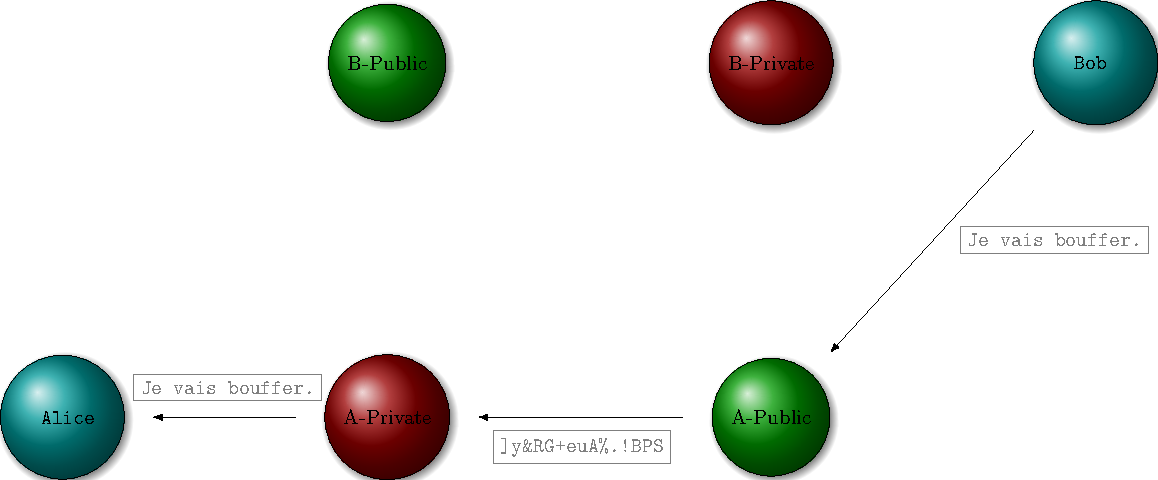
\includegraphics[scale=0.55]{res-src/asym_crypto_com}
    \end{center}
    \begin{itemize}
        \item Bob est sûr que Alice est la seule à pouvoir lire le message
        \item Alice ne sait pas qui est l'auteur du message
    \end{itemize}
\end{frame}

%------------------------------------------------

\begin{frame}
\frametitle{Réponse en clair de Alice avec Signature du message}
    \begin{center}
        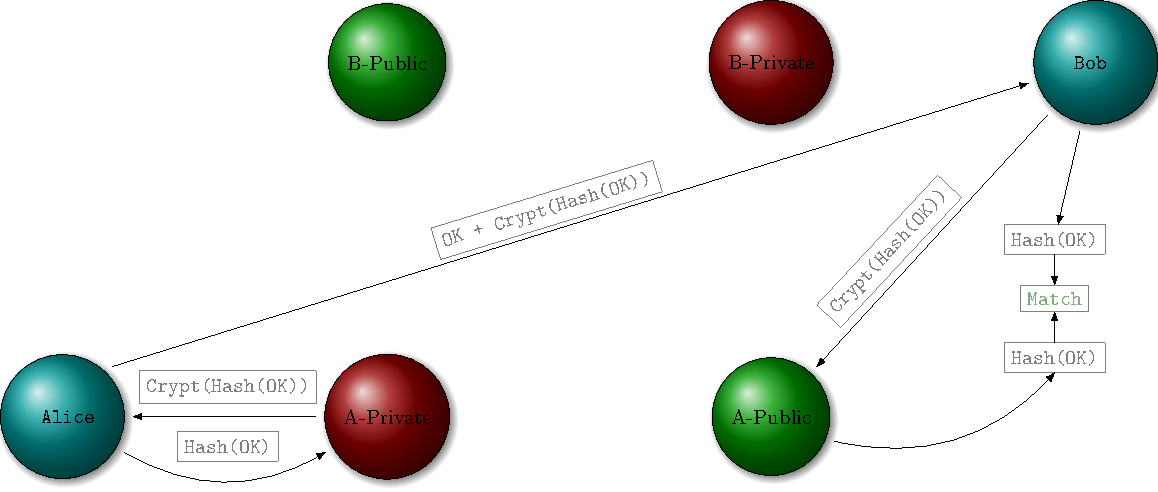
\includegraphics[scale=0.55]{res-src/asym_crypto_sign}
    \end{center}
    \begin{itemize}
        \item Alice envoie message en clair + hash chiffré par sa clef privée
        \item Bob déchiffre le hash de Alice, et calcule le hash de son côté
    \end{itemize}
\end{frame}
